\documentclass[11pt]{article}
\usepackage{aaHWbeginner}
\usepackage{tikz}
\usepackage{mathtools}
\usetikzlibrary{shapes,arrows,matrix,decorations.markings}
\newcommand*\circled[1]{\tikz[baseline=(char.base)]{
            \node[shape=circle,draw,inner sep=2pt] (char) {#1};}}
%%the \circled command has been used to create text inside circle for grading table.
\tikzstyle{blk}=[circle,inner sep=0pt,minimum size =2pt,draw,fill=black,line width=0.8pt]
\tikzstyle{blanknode}=[circle,inner sep=2pt,minimum size =8pt,draw,line width=0.8pt]
%%following is to have a directed edge with arrow anywhere in between, name of the style is ->- and it requres an input for the position of the arrow.
%%requires decorations.markings library
%% example usgae \draw[->-=0.5] (0,0) to [bend left] (2,4);
%% see http://tex.stackexchange.com/questions/39278/tikz-arrowheads-in-the-center
\tikzset{->-/.style={decoration={markings,mark=at position #1 with {\arrow{>}}},postaction={decorate}}}


%%%\geometry{letterpaper, textwidth=17cm, textheight=22cm}

%%%%%%%%%%%%%%%%%%%%%%%%%%%%%%%%%%%% THE FOLLOWING IS FOR THE COVER SHEET--FILL IN appropriately%%
\newcommand{\mycourse}{MATH-241}
\newcommand{\semesteryear}{Fall 2015}
\newcommand{\myname}{Matthew Gambogi}
\newcommand{\hwnumber}{1}
%%%%%%%%%%%%%%%%%%%%%%%%%%%%%%%%%%%%%% cover sheet preamble ends here

% following counter is to automate the numbering of the problems
\newcounter{Quesnumb}  % creates the counter
\setcounter{Quesnumb}{0} % sets a specific value to the counter
% the following new command can be used to increment and print the counter
% http://chenfuture.wordpress.com/2007/12/31/a-simple-counter/
\newcommand{\problemnum}{%
            \addtocounter{Quesnumb}{1}%
            \arabic{Quesnumb}}


\title{\textbf{\mycourse} \hfill Homework \hwnumber \hfill \textbf{\semesteryear}} %% DO NOT type in HW number here
\author{\myname}
\date{ \textbf{DUE DATE Sep 03, 2015 by 11:00PM (in \textsc{Dropbox})}}

%%%%%%%%%%%%%%%%%%%%%%%%%%%%%%%%%%%%%%%%%%%%%%%%%%%%%%%%%%%%%%%%%%%%%%%%%%%%%%%%%%%%%%%%%%%%%%%%%%%%%%%%%%%%%%%%%%%%%%%%%%%%%%%%

\setlength{\parindent}{0pt} %% paragraphs will not be indented
\setlength{\parskip}{.25cm} %% space between paragraphs
\linespread{1.1}

\begin{document}
\thispagestyle{empty} %%this is to supress the page number on the cover page
%% this file is for LaTeX users
%% the %% this file is for LaTeX users
%% the %% this file is for LaTeX users
%% the \include{hwcover} in the preamble of your HW file takes this file as an input and renders all the information appropriately.
%% this file should be in the same directory as your HW files.
%% DO NOT type your name etc. here in this file. See the preamble of your HW template file, where you need to write those inputs.
\newcommand{\circlescale}{& \circled{5} \hspace*{0.2cm} \circled{4} \hspace*{0.2cm} \circled{3} \hspace*{0.2cm} \circled{2} \hspace*{0.2cm} \circled{0}\\\midrule}
\begin{minipage}{6in}
    {\Large \mycourse \hfill Linear Algebra \hfill \semesteryear}
    \begin{center}
    %%\textsf{\huge Cover Sheet for HW}\\
    %%\vspace*{0.3cm}
    \fbox{\parbox[][1cm][c]{10cm}{\sc \Large Print Name: \myname}}
    \end{center}
\end{minipage}
\vspace*{0.3cm}

\textbf{Read the instructions below:}
\begin{itemize}
    %%\item \textsf{STAPLE} your homework.
    \item Solutions should be supported with reasons. Just writing the numerical answers is not enough and NO credit will be given for that.
    \item Please submit both the \LaTeX and PDF files. Refer to the instructions on the HW page about submitting the homework .
\end{itemize}

\begin{center}
\fbox{\parbox[][0.8cm][c]{10cm}{{\sc Assignment \# \hwnumber}}}
\end{center}

%%%for the \circled command used below see the file hw_template.tex. I have used TikZ to do this.

\renewcommand{\arraystretch}{1.3}
\begin{tabular}{lc}
  \toprule[2pt]
  % after \\: \midrule or \cline{col1-col2} \cline{col3-col4} ...
  \multicolumn{2}{c}{\bfseries For Grading Only}\\ \toprule[2pt]
  Completion Points \circlescale
  \#1               \circlescale
  \#2               \circlescale
  \#3               \circlescale
  \#4               \circlescale
  \#5               \circlescale
  \#6               \circlescale
  \#7               \circlescale
  \#8               \circlescale
  \#9               \circlescale
  \textbf{Total} & \\
  \bottomrule[2pt]
\end{tabular}
 in the preamble of your HW file takes this file as an input and renders all the information appropriately.
%% this file should be in the same directory as your HW files.
%% DO NOT type your name etc. here in this file. See the preamble of your HW template file, where you need to write those inputs.
\newcommand{\circlescale}{& \circled{5} \hspace*{0.2cm} \circled{4} \hspace*{0.2cm} \circled{3} \hspace*{0.2cm} \circled{2} \hspace*{0.2cm} \circled{0}\\\midrule}
\begin{minipage}{6in}
    {\Large \mycourse \hfill Linear Algebra \hfill \semesteryear}
    \begin{center}
    %%\textsf{\huge Cover Sheet for HW}\\
    %%\vspace*{0.3cm}
    \fbox{\parbox[][1cm][c]{10cm}{\sc \Large Print Name: \myname}}
    \end{center}
\end{minipage}
\vspace*{0.3cm}

\textbf{Read the instructions below:}
\begin{itemize}
    %%\item \textsf{STAPLE} your homework.
    \item Solutions should be supported with reasons. Just writing the numerical answers is not enough and NO credit will be given for that.
    \item Please submit both the \LaTeX and PDF files. Refer to the instructions on the HW page about submitting the homework .
\end{itemize}

\begin{center}
\fbox{\parbox[][0.8cm][c]{10cm}{{\sc Assignment \# \hwnumber}}}
\end{center}

%%%for the \circled command used below see the file hw_template.tex. I have used TikZ to do this.

\renewcommand{\arraystretch}{1.3}
\begin{tabular}{lc}
  \toprule[2pt]
  % after \\: \midrule or \cline{col1-col2} \cline{col3-col4} ...
  \multicolumn{2}{c}{\bfseries For Grading Only}\\ \toprule[2pt]
  Completion Points \circlescale
  \#1               \circlescale
  \#2               \circlescale
  \#3               \circlescale
  \#4               \circlescale
  \#5               \circlescale
  \#6               \circlescale
  \#7               \circlescale
  \#8               \circlescale
  \#9               \circlescale
  \textbf{Total} & \\
  \bottomrule[2pt]
\end{tabular}
 in the preamble of your HW file takes this file as an input and renders all the information appropriately.
%% this file should be in the same directory as your HW files.
%% DO NOT type your name etc. here in this file. See the preamble of your HW template file, where you need to write those inputs.
\newcommand{\circlescale}{& \circled{5} \hspace*{0.2cm} \circled{4} \hspace*{0.2cm} \circled{3} \hspace*{0.2cm} \circled{2} \hspace*{0.2cm} \circled{0}\\\midrule}
\begin{minipage}{6in}
    {\Large \mycourse \hfill Linear Algebra \hfill \semesteryear}
    \begin{center}
    %%\textsf{\huge Cover Sheet for HW}\\
    %%\vspace*{0.3cm}
    \fbox{\parbox[][1cm][c]{10cm}{\sc \Large Print Name: \myname}}
    \end{center}
\end{minipage}
\vspace*{0.3cm}

\textbf{Read the instructions below:}
\begin{itemize}
    %%\item \textsf{STAPLE} your homework.
    \item Solutions should be supported with reasons. Just writing the numerical answers is not enough and NO credit will be given for that.
    \item Please submit both the \LaTeX and PDF files. Refer to the instructions on the HW page about submitting the homework .
\end{itemize}

\begin{center}
\fbox{\parbox[][0.8cm][c]{10cm}{{\sc Assignment \# \hwnumber}}}
\end{center}

%%%for the \circled command used below see the file hw_template.tex. I have used TikZ to do this.

\renewcommand{\arraystretch}{1.3}
\begin{tabular}{lc}
  \toprule[2pt]
  % after \\: \midrule or \cline{col1-col2} \cline{col3-col4} ...
  \multicolumn{2}{c}{\bfseries For Grading Only}\\ \toprule[2pt]
  Completion Points \circlescale
  \#1               \circlescale
  \#2               \circlescale
  \#3               \circlescale
  \#4               \circlescale
  \#5               \circlescale
  \#6               \circlescale
  \#7               \circlescale
  \#8               \circlescale
  \#9               \circlescale
  \textbf{Total} & \\
  \bottomrule[2pt]
\end{tabular}
 %% make sure you have the file "hwcover.tex" in the same folder as your actual homework file
\renewcommand{\arraystretch}{1} %% this is to make sure that array stretch in "hwcover" is nuetralized.

\clearpage %% these are to reset the page number for the first page of your homework to 1.
\pagenumbering{arabic} %% these are to reset the page number for the first page of your homework to 1.
\maketitle

% Use the ``problem'' environment for questions and the ``solution'' environment to type the solutions.

\begin{problem}{\problemnum \, \textsf{(POOLE 2.3.12)}}
    Show that $\bbR^3$ = span$\parens{\vvv{ 1}{ 1}{-1}
                                      \vvv{ 1}{ 1}{ 1}
                                      \vvv{ 1}{-1}{ 1}}$.
\end{problem}
\begin{solution}

\end{solution}

\begin{problem}{\problemnum \, \textsf{(POOLE 2.3.16)}}
    Describe the set of given vectors (a) geometrically, and (b) algebraically.
    $$ \vvv{  }{  }{ }
       \vvv{  }{  }{ }
       \vvv{  }{  }{ }
    $$
\end{problem}
\begin{solution}
\end{solution}

\begin{problem}{\problemnum \, \textsf{(POOLE 1.2.48)}}
    Find all values of the scalar $k$ for which the two
    vectors are orthagonal
    \[ \bu = \vect{2}{3},
        \bv = \vect{k + 1}{k - 1}
    \]
\end{problem}
\begin{solution}\\
    In $\mathbb{R}^2$:
    \[ \frac{\bu \cdot \bv}
            {\norm*{\bu} \norm*{\bv}}
        = \cos(\pi/2)
        = 0
        \implies \bu \text{ is perpendicular to } \bv
    \]
    Reifiying, we have:
    \begin{align*}
        \frac{\vect{2}{3} \cdot \vect{k+1}{k-1}}
             {\norm*{\vect{2}{3}}\norm*{\vect{k+1}{k-1}}} &= 0
        \\\\
        \frac{2k + 2 + 3k - 3}
             {\sqrt{13}\sqrt{(k + 1)^{2} + (k - 1)^{2}}} &= 0
        \\\\
        \frac{5k - 1}
             { \sqrt{13}\sqrt{2k^{2} + 2}} &= 0
        \\\\
        \frac{5k - 1}
             {\sqrt{2}\sqrt{13}\sqrt{k^2 + 1}} &= 0
        \\\\
        \frac{5k - 1}
             {\sqrt{k^2 + 1}} &= 0
        \\\\
        \frac{5k}{\sqrt{k^2 + 1}}
        &=
        \frac{1}{\sqrt{k^2 + 1}}
        \\\\
        5k &= 1
        \\\\
        k &= \frac{1}{5}
    \end{align*}
\end{solution}

\begin{problem}{\problemnum \, \textsf{(POOLE 2.3.24)}}

\end{problem}


\begin{problem}{\problemnum \, \textsf{(POOLE 2.3.30)}}

\end{problem}

\begin{problem}{\problemnum} 
Let $\bv$ and $\bw$ be vectors in $\bbR^{n}$. If $\norm{\bv}=5$ and $\norm{\bw}=3$, what are the largest and smallest values of $\norm{\bv-\bw}$? What are the largest and smallest values of $\bv \cdot \bw$?
\end{problem}
\begin{solution}
    By Cauchy-Sharz-Bunyakowski:
    \[\abs{\bv \cdot \bw} \le \norm{\bv}\norm{\bw}\]
    Substituting:
    \[ 0 \le \abs{\bv \cdot \bw} \le 15 \]
    Therefore:
    \[ -15 \le \bv \cdot \bw \le 15 \]
    Now:
    \begin{align*}
        \norm{\bv - \bw} &= \sqrt{(\bv - \bw)(\bv - \bw)}
        \\\\
        &= \sqrt{\bv \cdot \bv - 2(\bv \cdot \bw) + \bw \cdot \bw}
        \\\\
        &= \sqrt{25 - 2(\bv \cdot \bw) + 9}
        \\\\
        &= \sqrt{34 - 2(\bv \cdot \bw)}
        \\\\
        &= \sqrt{2}\sqrt{17 - \bv \cdot \bw}
    \end{align*}
    It follows:
    \[  \sqrt{2}\sqrt{17 - \min(\bv \cdot \bw)}
    \le \norm{\bv - \bw}
    \le \sqrt{2}\sqrt{17 - \max(\bv \cdot \bw)}
    \]
    Substituting:
    \[  \sqrt{2}\sqrt{17 - 15}
    \le \norm{\bv - \bw}
    \le \sqrt{2}\sqrt{17 + 15}
    \]
    Therefore:
    \[  2\sqrt{2}
    \le \norm{\bv - \bw}
    \le 5\sqrt{2}
    \]
\end{solution}

\begin{problem}{\problemnum} 
Let $\bu, \bv, \bw$ be vectors such that $\norm{\bu}=1, \norm{\bv}=2$ and $\norm{\bw}=3$, $\bu$ is orthogonal to $\bv$, and that the angle between $\bu$ and $\bw$ is $\pi/3$ and that between $\bv$ and $\bw$ is $\pi/6$. Find $\norm{\bu+\bv+\bw}$.
\end{problem}
\begin{solution}\\
    Solving for $\bu \cdot \bv$:
    \begin{align*}
        & \frac{\bu \cdot \bv}
               {\norm{\bu}\norm{\bv}} = 0 = \cos(\frac{\pi}{2})
        \\
        \implies& \bu \cdot \bv = 0
    \end{align*}
    Solving for $\bu \cdot \bw$:
    \begin{align*}
        & \frac{\bu \cdot \bw}
        {\norm{\bu}\norm{\bw}} = \frac{1}{2} = \cos(\frac{\pi}{3})
        \\
        \implies& \bu \cdot \bw = \frac{3}{2}
    \end{align*}
    Solving for $\bu \cdot \bw$:
    \begin{align*}
        & \frac{\bv \cdot \bw}
        {\norm{\bv}\norm{\bw}} = \frac{\sqrt{3}}{2} = \cos(\frac{\pi}{6})
        \\
        \implies& \bv \cdot \bw = 3\sqrt{3}
    \end{align*}
    Rewriting $\norm{\bu+\bv+\bw}$
    \begin{align*}
        & \norm{\bu+\bv+\bw}
        \\
        =& \sqrt{(\bu+\bv+\bw) \cdot (\bu+\bv+\bw)}
        \\
        =& \sqrt{\bu \cdot (\bu+\bv+\bw)
                      + \bv \cdot (\bu+\bv+\bw)
                      + \bw \cdot (\bu+\bv+\bw)}
        \\
        =& \sqrt{\bu \cdot \bu
                      + \bv \cdot \bv
                      + \bw \cdot \bw
                      + 2(\bu \cdot \bv)
                      + 2(\bu \cdot \bw)
                      + 2(\bv \cdot \bw)}
        \\
        =& \sqrt{\norm{\bu}^{2}
                      + \norm{\bv}^{2}
                      + \norm{\bw}^{2}
                      + 2(\bu \cdot \bv)
                      + 2(\bu \cdot \bw)
                      + 2(\bv \cdot \bw)}
        \\
        =& \sqrt{1^2 + 2^2 + 3^2 + 2(0) + 2(3/2) + 2(3\sqrt{3})}
        \\
        =& \sqrt{17+6\sqrt{3}}
    \end{align*}

\end{solution}

\begin{problem}{\problemnum} 
Let $A$ and $B$ be the endpoints of a diameter of a circle and $O$ be the center (without the loss of generality we can place it at the origin). Suppose $C$ is any point on the circle (see the figure below). Let the position vectors of $A$ be $\ba$ and that of $C$ be $\bc$. Using this prove that $\angle ACB$ is a right angle. \textsf{Hint:} Try to express the vectors $\overrightarrow{AC}$ and $\overrightarrow{CB}$ in terms of $\ba$ and $\bc$.\\
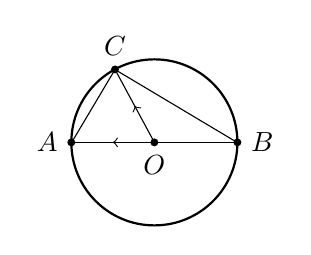
\begin{tikzpicture}
    \draw[thick] (0,0) circle (30pt);
    \draw (-1.05,0) -- (1.05,0);
    \draw (-1.05,0) -- (-0.5,0.925) --(1.05,0);
    \node[style=blk, label=left:$A$](A) at (-1.055,0){};
    \node[style=blk, label=right:$B$](B) at (1.055,0){};
    \node[style=blk, label=above:$C$](C) at (-.5,0.926){};
    \node[style=blk, label=below:$O$](O) at (0,0){};
    \draw[->-=0.5] (O) to (A);
    \draw[->-=0.5] (O) to (C);
    \node (a) at (-0.55,-0.2) {$\scriptstyle \ba$};
    \node (c) at (-0.45,0.4) {$\scriptstyle \bc$};
\end{tikzpicture}
\end{problem}
\begin{solution}
    \begin{proof}
        \[\norm{\ba} = \norm{\bb} = \norm{\bc}\]
        \[\overrightarrow{AC} = \ba - \bc\]
        \[\overrightarrow{CB} = \bc + \ba\]
        \[\cos(\angle ABC) = \frac{(\ba - \bc) \cdot (\bc + \ba)}
                                  {\norm{\ba - \bc}\norm{\bc + \ba}}
                              \]
        \[\cos(\angle ABC) = \frac{(\ba \cdot \ba - \bc \cdot \bc)}
                                  {\norm{\ba - \bc}\norm{\bc + \ba}}
        \]
        \[\cos(\angle ABC) = \frac{\norm{\ba}^2 - \norm{\bc}^2}
                                  {\norm{\ba - \bc}\norm{\bc + \ba}}
        \]
        \[\cos(\angle ABC) = \frac{0}
                                  {\norm{\ba - \bc}\norm{\bc + \ba}}
        \]
        \[\cos(\angle ABC) = 0\]
        \[\angle ABC = \frac{\pi}{2}\]
        $\angle ABC$ must be perpendicular.

    \end{proof}
\end{solution}

\begin{problem}{\problemnum}
Let $\bA$ be a $7 \times 4$ matrix with linearly independent columns and $\bR$ be the row reduced echelon form of $\bA$.
    \begin{enumerate}
        \item Find the number of zero rows of $\bR$. Support your answer with reasons.
        \item Based on the information given complete the following sentence: \textsf{the columns of $\bA$ will span a \makebox[0.5in]{\hrulefill} dimensional space in a \makebox[0.5in]{\hrulefill} dimensional ambient space.}
        \item What can be said about the linear span of the rows of $\bA$ (be careful: rows of $\bA$ live in a different world than the columns)?
        \item Explain why $\bA^{T}\by = \begin{pmatrix}0&1&0&1\end{pmatrix}^{T}$ is a consistent system.
    \end{enumerate}
\end{problem}

\begin{problem}{\problemnum}
Let $\bA$ be a $123 \times 56$ matrix of rank $22$.
\begin{enumerate}
    \item How many independent vectors will satisfy the homogeneous equation $\bA\bx=\mathbf{0}$.
    \item How many independent vectors will satisfy the homogeneous equation $\bA^{T}\bx=\mathbf{0}$.
\end{enumerate}
\end{problem}

\begin{problem}{\problemnum} 
Let $\bu=\begin{pmatrix}
                 1 \\
                 1 \\
                 1  \\
                 \vdots \\
                 1
               \end{pmatrix}$ and $\bv=\begin{pmatrix}
                 1 \\
                 2 \\
                 3  \\
                 \vdots \\
                 n
               \end{pmatrix}$
               be two vectors in $\bbR^n$. Let $\theta_n$ be the angle between $\bu$ and $\bv$ in $\bbR^n$.
               \begin{enumalph}
                \item Find $\theta_n$.
                \item What will be $\lim_{n \to \infty} \theta_n$? Give a mathematical justification.
               \end{enumalph}
\end{problem}
\begin{solution}

\begin{align*}
    \cos(\theta_{n}) = \frac{\bu \cdot \bv}{\norm{\bu}\norm{\bv}}
    \\\\
    \bu \cdot \bv = 1(1) + 2(1) + ... + n(1) 
                  = 1 + 2 + ... + n
                  = \frac{n(n+1)}{2}
   \\\\
   \norm{\bu} = \sqrt{1^2 + ... + 1^2} = \sqrt{n}
   \\\\
   \norm{\bv} = \sqrt{1^2 + 2^2 + ... + n^2}
   = \sqrt{\frac{n(n+1)(2n+1}{6}}
   \\\\
   \cos(\theta_{n}) = \frac{\frac{n(n+1)}{2}}{\sqrt{n}\sqrt{\frac{n(n+1)(2n+1}{6}}}
   \\\\
   \cos(\theta_{n}) = \frac{\sqrt{6}}{2}\sqrt{\frac{n+1}{2n+1}}
   \\\\
   \theta_{n} = \cos^{-1}(\frac{\sqrt{6}}{2}\sqrt{\frac{n+1}{2n+1}})
   \\\\
   \lim_{n\to\inf}\cos^{-1}( \frac{\sqrt{6}} {2} \sqrt{\frac{n+1} {2n+1}}) &= \cos^{-1}\frac{\sqrt{6}}{2\sqrt{2}}
   \\
   &= \cos^{-1}\frac{\sqrt{3}}{2} 
   \\
   &= \frac{\pi}{6}
\end{align*}

\end{solution}


\end{document}
